\chapter{Background} \label{chp::bg}

For self-containedness, we provide a short references to the mathematical tools
that we have been frequently used in PLVMs. Readers familiar with the theory of
conjugate duality and EM algorithm can skip the content of this chapter. And for
a comprehensive account, please refer to the book \cite{hiriart1993convex}.

\section{Conjugate Duality}

The conjugate in optimization context refers to the transformation of a problem
to another accompanying problem. The transformation is also known as the
\emph{conjugacy} operation or the \emph{Legendre-Fenchel} transformation.  It
plays an important role in the Lagrangian duality as well as the general convex
optimization. To start our discussion, we formally define the conjugate of a
function as:

\begin{dfn}

  The conjugate of a convex function~\footnote{we make a stronger assumption
  that $f$ is convex which can relaxed to the existence of a affine function
  memorizing $f$ on $\mathrm{dom}\, f$.} $f$ is the function $f^*$ defined by

  \begin{equation}
    f^*(s) = \sup \{ \langle s, x \rangle - f(x) \}, \quad
    \forall x \in \mathrm{dom}\, f
  \end{equation}

\end{dfn}


\begin{figure}[h!]
  \centering
  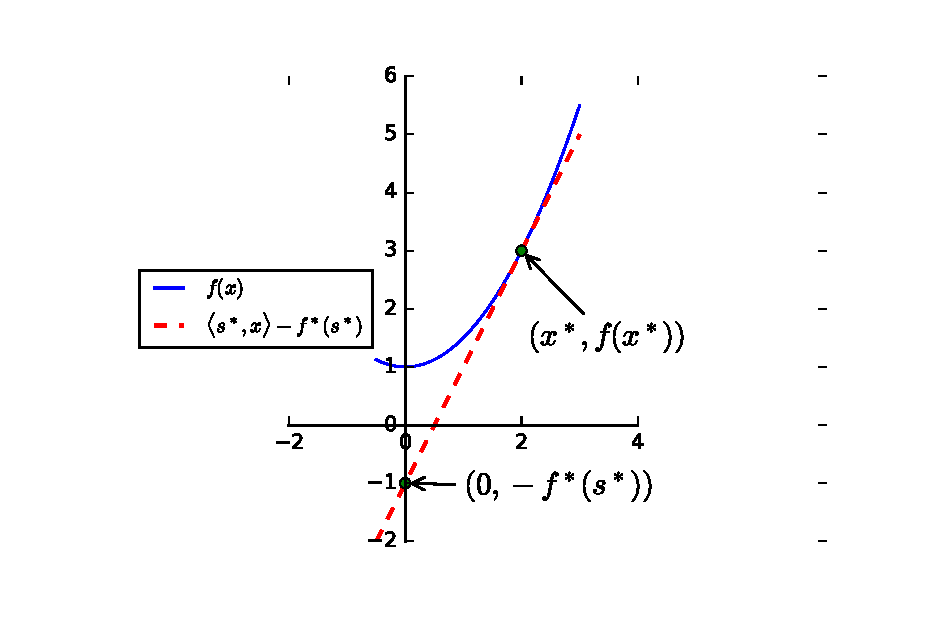
\includegraphics[width=0.7\linewidth, trim={0 0 3cm 1.5cm},
                    clip]{figures/conjugate-function.eps}

  \caption{A illustration of the relationship between $f$ and its conjugate
    $f^*$. For a given $s^*$, since $f(x) \geq \langle s^*, x \rangle  -
    f^*(s^*)$ always holds, which means that in the plot the curve of $f(x)$ is
    always above (or on) the line of $\langle s^*, x \rangle  - f^*(s^*)$. As a
    limiting case, $<s^*, x^*> - f^*(s^*)$ is cutting $f(x)$ at $x = x^*$. In
    addition, the affine function intersects the vertical axis $x = 0$ at the
    altitude $-f^*(s^*)$. The plot also shows the relationship between $s^*$ and
    $x^*$ can be described by the \emph{gradient mapping}: $x^* \in \partial
    f^{-1}(s^*)$.}

  \label{fig::conjugate-function}
\end{figure}

An geometrical interpretation of the conjugate of a \emph{subdifferentiable}
function is illustrated in Figure~\ref{fig::conjugate-function}. A immediate
result is that:

\begin{thm} \label{thm::conjugate-attainer}
For any $x^* \in \argmax \{ \langle s^*, x \rangle  - f^*(s^*)
\}$, we have that $x^* \in \partial f^{-1}(s^*)$
\end{thm}

In addition, the conjugacy transformation is in general symmetric: $f^{**} = f$
for convex functions. To be exact, the identity between the bi-conjugate
$f^{**}$ and $f$ is equivalent to the requirement that the convex $f$ is
lower semi-continuity (l.s.c): $\liminf\limits_{x \rightarrow x_0} \geq f(x_0)$,
a sufficient condition of which is that $f$ is subdifferentiablen.

\subsubsection{Log-Partition and Negative Entropy}

One important instance of the conjugate in PLVMs is between log-partition and
negative entropy, which are defined as below:

\begin{alignat}{-1}
  &\text{Log-Parition:} & \quad
  A(\mathbf{x}) &= \log \sum\limits_{i = 1}^N \exp(x_i) \\
  &\text{Negative Entropy:} & \quad
  - H(\mathbf{p}) &= \sum\limits_{i = 1}^N p_i \log p_i
\end{alignat}
where the $\mathbf{p}$ is an element in the simplex set which is defined as:
$$\Delta_N = \{\mathbf{p} \in
  \mathbb{R}^{N}: p_j \ge 0, \sum\limits_{j=1}^N p_j = 1\}$$

The log-partition function is often seen in Maximum Entropy model, energy-based
model, as well as Markov Random Fields, \etc. The straight-forward computation
involves a summation over $N$ items, which can be computational challenging if
$N$ is large. For example, in Markov Random Fields, $N = m!$  where is $m$ is
the number of nodes in the random fields, and therefore computing the
log-partition function is the bottleneck for training such a model.

It is easy to verify that both function is convex and smooth. Their connection
is presented in the theorem below.

\begin{lem} \label{lem::conj_dual}
  Assume that
  $$\P(i; \vs) = \frac{\exp(s_i)}{\sum\limits_{j=1}^N \exp(s_j)}$$
  and
  $$A(\vs) = \log \sum\limits_{j = 1}^N \exp(s_j)$$
  The conjugate duality between the log-partition function and negative entropy
  states:
  \begin{align}
    A(\vs) &= \max\limits_{\vmu \in \Delta_N}
                    \{ \sum\limits_{j=1}^N \mu_j s_j -
                       \sum\limits_{j=1}^N \mu_j \log \mu_j \} \nonumber \\
           &= \max\limits_{\vmu \in \Delta_N}
                    \{ \E_{\vmu} [s_j] + \entropy(\vmu) \} \label{eq::conj_dual}
  \end{align}
  where the maximizer is attained at:
  \begin{align}
    \mu_j^* = \P(j; \vs), \quad 1 \le j \le N \label{eq::conj_dual_sol}
  \end{align}
\end{lem}
\begin{proof}

  In light of Theorem~\ref{thm::conjugate-attainer}, the general proof of the
  conjugacy transformation between $f$ and $f^*$ is to verify that $x = \partial
  f^* \big( \partial f(x) \big)$. And it is easy to show that

  $$\vs = -\partial H \big(\partial A (\vs) \big)$$

  However, it is much more intuitive to equivalence in
  \Cref{eq::conj_dual_sol} We use the following equivalence:

  \begin{align*}
    \E_{\vmu}[s_j] + \entropy(\vmu)
      &= -\sum\limits_{j=1}^N \mu_j \log \frac{\mu_j }{ \P(j; \vs) } +
          \log\sum\limits_{j=1}^N \exp(s_j) \nonumber \\
      &= -D_{KL}(\vmu || \P) + A(\vs)
  \end{align*}
where $D_{KL}(\vmu || \P)$ is the Kullback-Leibler (KL) divergence and
note $D_{KL}(\vmu || P) \ge 0$ and $D_{KL}(P || P) = 0$.
It follows that
$\vmu^* = \argmin\limits_{\vmu \in \Delta_N} D_{KL}(\vmu || P) = P$.
\end{proof}

\section{Minimax Theory}
\section{EM Algorithm: a modern reinterpretation} \label{sec::bg-em}
